
\section{模的\trLifting{}与\trExtension}\label{sec:liftings-and-extensions-of-modules}

在本节中，我们在模的\trVirtualEquipment{}中引入并研究\trLifting{}与%
\trExtension{}。为给\cref{def:right-extension-lifting-modules}提供动机，我们
先简要回忆那个标准的 2-范畴式概念：

\begin{definition}\label{def:two-categorical-extension}
1-\trCell{} $f\colon A\to C$ 沿 1-\trCell{} $k\colon A\to B$ 的一个%
\textbf{右扩张}（right extension），由一个数对
$(r\colon B\to C,\ \nu\colon rk\Rightarrow f)$ 给出，如下左图所示
\begin{center}
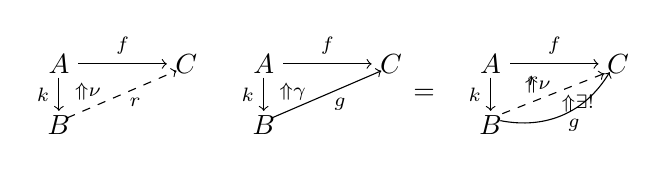
\begin{tikzpicture}[x=1em,y=1em]
  \node at (0,2.2)   {$A$};
  \node at (4.6,2.2) {$C$};
  \node at (0,0)     {$B$};
  \draw[->] (0.7,2.2) -- node[above]{$\scriptstyle f$} (3.9,2.2);
  \draw[->] (0,1.7)   -- node[left]{$\scriptstyle k$} (0,0.5);
  \draw[->,dashed] (0.3,0.25) -- node[below,pos=0.62]{$\scriptstyle r$} (4.25,1.95);
  \node at (1.05,1.2) {$\scriptstyle\Uparrow\nu$};
  \begin{scope}[shift={(7.4,0)}]
    \node at (0,2.2)   {$A$};
    \node at (4.6,2.2) {$C$};
    \node at (0,0)     {$B$};
    \draw[->] (0.7,2.2) -- node[above]{$\scriptstyle f$} (3.9,2.2);
    \draw[->] (0,1.7)   -- node[left]{$\scriptstyle k$} (0,0.5);
    \draw[->] (0.3,0.25) -- node[below,pos=0.62]{$\scriptstyle g$} (4.25,1.95);
    \node at (1.05,1.2) {$\scriptstyle\Uparrow\gamma$};
  \end{scope}
  \node at (13.2,1.1) {$=$};
  \begin{scope}[shift={(15.6,0)}]
    \node at (0,2.2)   {$A$};
    \node at (4.6,2.2) {$C$};
    \node at (0,0)     {$B$};
    \draw[->] (0.7,2.2) -- node[above]{$\scriptstyle f$} (3.9,2.2);
    \draw[->] (0,1.7)   -- node[left]{$\scriptstyle k$} (0,0.5);
    \draw[->,dashed] (0.42,0.4) -- node[above left,pos=0.45]{$\scriptstyle r$} (4.1,1.85);
    \draw[->] (0.35,0.15) to[bend right=35] node[below,pos=0.6]{$\scriptstyle g$} (4.3,1.9);
    \node at (1.7,1.45)  {$\scriptstyle\Uparrow\nu$};
    \node at (3.15,0.75) {$\scriptstyle\Uparrow\exists!$};
  \end{scope}
\end{tikzpicture}
\end{center}
使得任何如中图所示的那类数对都经由 $\nu$ 唯一地分解，如上右图所示。

对偶地，1-\trCell{} $f\colon A\to C$ 沿 1-\trCell{} $k\colon A\to B$ 的一个%
\textbf{左扩张}（left extension），由一个数对
$(\ell\colon B\to C,\ \lambda\colon f\Rightarrow \ell k)$ 给出，如下左图所示
\begin{center}
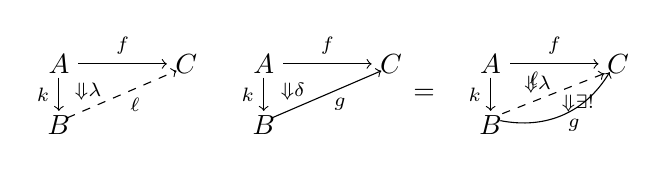
\begin{tikzpicture}[x=1em,y=1em]
  \node at (0,2.2)   {$A$};
  \node at (4.6,2.2) {$C$};
  \node at (0,0)     {$B$};
  \draw[->] (0.7,2.2) -- node[above]{$\scriptstyle f$} (3.9,2.2);
  \draw[->] (0,1.7)   -- node[left]{$\scriptstyle k$} (0,0.5);
  \draw[->,dashed] (0.3,0.25) -- node[below,pos=0.62]{$\scriptstyle\ell$} (4.25,1.95);
  \node at (1.05,1.2) {$\scriptstyle\Downarrow\lambda$};
  \begin{scope}[shift={(7.4,0)}]
    \node at (0,2.2)   {$A$};
    \node at (4.6,2.2) {$C$};
    \node at (0,0)     {$B$};
    \draw[->] (0.7,2.2) -- node[above]{$\scriptstyle f$} (3.9,2.2);
    \draw[->] (0,1.7)   -- node[left]{$\scriptstyle k$} (0,0.5);
    \draw[->] (0.3,0.25) -- node[below,pos=0.62]{$\scriptstyle g$} (4.25,1.95);
    \node at (1.05,1.2) {$\scriptstyle\Downarrow\delta$};
  \end{scope}
  \node at (13.2,1.1) {$=$};
  \begin{scope}[shift={(15.6,0)}]
    \node at (0,2.2)   {$A$};
    \node at (4.6,2.2) {$C$};
    \node at (0,0)     {$B$};
    \draw[->] (0.7,2.2) -- node[above]{$\scriptstyle f$} (3.9,2.2);
    \draw[->] (0,1.7)   -- node[left]{$\scriptstyle k$} (0,0.5);
    \draw[->,dashed] (0.42,0.4) -- node[above left,pos=0.45]{$\scriptstyle\ell$} (4.1,1.85);
    \draw[->] (0.35,0.15) to[bend right=35] node[below,pos=0.6]{$\scriptstyle g$} (4.3,1.9);
    \node at (1.7,1.45)  {$\scriptstyle\Downarrow\lambda$};
    \node at (3.15,0.75) {$\scriptstyle\Downarrow\exists!$};
  \end{scope}
\end{tikzpicture}
\end{center}
使得任何如中图所示的那类数对都经由 $\lambda$ 唯一地分解，如上右图所示。
\end{definition}

\cref{def:two-categorical-extension}的诸 op-对偶在任何 2-范畴中定义了%
\textbf{右\trLifting}（right lifting）与\textbf{左\trLifting}（left lifting）图。
对于\trVirtualDoubleCategory{}中的水平箭头，也能定义类似的右扩张与右提升
概念；而凡当\trVirtualEquipment{}拥有其限制（restriction）时，只需考虑那些
竖直边缘箭头皆为恒同的「纤维化」胞腔便已足够。
我们于是把用语专门化到模的\trVirtualEquipment{}，因为这正是我们感兴趣的
场合：

\begin{definition}\label{def:right-extension-lifting-modules}
模 $A\xrightarrow{F}C$ 沿模 $A\xrightarrow{K}B$ 的一个\textbf{右扩张}，由
一支模 $B\xrightarrow{R}C$ 连同一个二元\trCell{}一起构成的数对给出
\begin{center}
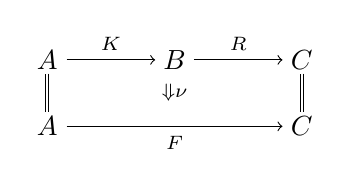
\begin{tikzpicture}[x=1em,y=1em]
  \node at (0,1.2)    {$A$};
  \node at (4.6,1.2)  {$B$};
  \node at (9.2,1.2)  {$C$};
  \node at (0,-1.2)   {$A$};
  \node at (9.2,-1.2) {$C$};
  \draw[->] (0.7,1.2)  -- node[above]{$\scriptstyle K$} (3.9,1.2);
  \draw[->] (5.3,1.2)  -- node[above]{$\scriptstyle R$} (8.5,1.2);
  \draw[->] (0.7,-1.2) -- node[below]{$\scriptstyle F$} (8.5,-1.2);
  \draw[double] (0,0.7)   -- (0,-0.7);
  \draw[double] (9.2,0.7) -- (9.2,-0.7);
  \node at (4.6,0) {$\scriptstyle\Downarrow\nu$};
\end{tikzpicture}
\end{center}
它具有如下性质：每一个形如下左图所示的 $n+1$ 元\trCell{}都经由
$\nu\colon K\divideontimes R\Rightarrow F$ 唯一地分解，如下右图所示：
\begin{center}
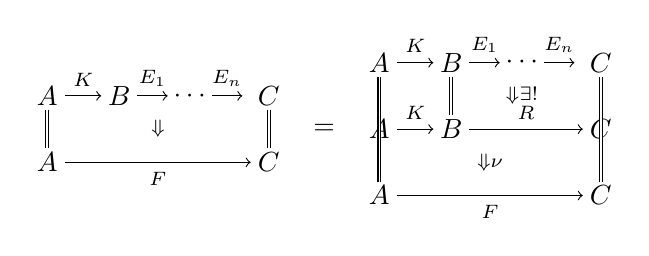
\begin{tikzpicture}[x=1em,y=1em]
  \begin{scope}
    \node at (0,1.2)   {$A$};
    \node at (2.6,1.2) {$B$};
    \node at (8.0,1.2) {$C$};
    \draw[->] (0.65,1.2) -- node[above]{$\scriptstyle K$} (1.95,1.2);
    \draw[->] (3.25,1.2) -- node[above]{$\scriptstyle E_{1}$} (4.35,1.2);
    \node at (5.15,1.2)  {$\cdots$};
    \draw[->] (5.95,1.2) -- node[above]{$\scriptstyle E_{n}$} (7.05,1.2);
    \node at (0,-1.2)    {$A$};
    \node at (8.0,-1.2)  {$C$};
    \draw[->] (0.65,-1.2) -- node[below]{$\scriptstyle F$} (7.35,-1.2);
    \draw[double] (0,0.7)   -- (0,-0.7);
    \draw[double] (8.0,0.7) -- (8.0,-0.7);
    \node at (4.0,0) {$\scriptstyle\Downarrow$};
  \end{scope}
  \node at (10.0,0) {$=$};
  \begin{scope}[shift={(12.0,0)}]
    \node at (0,2.4)   {$A$};
    \node at (2.6,2.4) {$B$};
    \node at (8.0,2.4) {$C$};
    \draw[->] (0.65,2.4) -- node[above]{$\scriptstyle K$} (1.95,2.4);
    \draw[->] (3.25,2.4) -- node[above]{$\scriptstyle E_{1}$} (4.35,2.4);
    \node at (5.15,2.4)  {$\cdots$};
    \draw[->] (5.95,2.4) -- node[above]{$\scriptstyle E_{n}$} (7.05,2.4);
    \node at (0,0)   {$A$};
    \node at (2.6,0) {$B$};
    \node at (8.0,0) {$C$};
    \draw[->] (0.65,0) -- node[above]{$\scriptstyle K$} (1.95,0);
    \draw[->] (3.25,0) -- node[above]{$\scriptstyle R$} (7.35,0);
    \node at (0,-2.4)   {$A$};
    \node at (8.0,-2.4) {$C$};
    \draw[->] (0.65,-2.4) -- node[below]{$\scriptstyle F$} (7.35,-2.4);
    \draw[double] (0,1.9)   -- (0,-1.9);
    \draw[double] (8.0,1.9) -- (8.0,-1.9);
    \draw[double] (2.6,1.9) -- (2.6,0.5);
    \node at (5.15,1.2) {$\scriptstyle\Downarrow\exists!$};
    \node at (4.0,-1.2) {$\scriptstyle\Downarrow\nu$};
  \end{scope}
\end{tikzpicture}
\end{center}

对偶地，模 $A\xrightarrow{F}C$ 穿过模 $B\xrightarrow{H}C$ 的一个%
\textbf{右提升}，由一支模 $A\xrightarrow{L}B$ 连同一个二元\trCell{}一起构成
的数对给出
\begin{center}
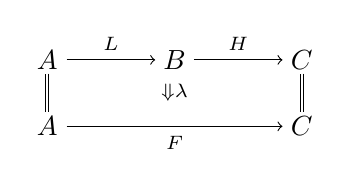
\begin{tikzpicture}[x=1em,y=1em]
  \node at (0,1.2)    {$A$};
  \node at (4.6,1.2)  {$B$};
  \node at (9.2,1.2)  {$C$};
  \node at (0,-1.2)   {$A$};
  \node at (9.2,-1.2) {$C$};
  \draw[->] (0.7,1.2)  -- node[above]{$\scriptstyle L$} (3.9,1.2);
  \draw[->] (5.3,1.2)  -- node[above]{$\scriptstyle H$} (8.5,1.2);
  \draw[->] (0.7,-1.2) -- node[below]{$\scriptstyle F$} (8.5,-1.2);
  \draw[double] (0,0.7)   -- (0,-0.7);
  \draw[double] (9.2,0.7) -- (9.2,-0.7);
  \node at (4.6,0) {$\scriptstyle\Downarrow\lambda$};
\end{tikzpicture}
\end{center}
它具有如下性质：每一个形如下左图所示的 $n+1$ 元\trCell{}都经由
$\lambda\colon L\divideontimes H\Rightarrow F$ 唯一地分解，如下右图所示：
\begin{center}
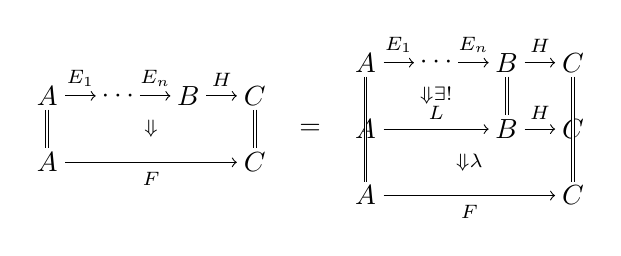
\begin{tikzpicture}[x=1em,y=1em]
  \begin{scope}
    \node at (0,1.2)   {$A$};
    \node at (5.1,1.2) {$B$};
    \node at (7.5,1.2) {$C$};
    \draw[->] (0.65,1.2) -- node[above]{$\scriptstyle E_{1}$} (1.75,1.2);
    \node at (2.55,1.2)  {$\cdots$};
    \draw[->] (3.35,1.2) -- node[above]{$\scriptstyle E_{n}$} (4.45,1.2);
    \draw[->] (5.75,1.2) -- node[above]{$\scriptstyle H$} (6.85,1.2);
    \node at (0,-1.2)    {$A$};
    \node at (7.5,-1.2)  {$C$};
    \draw[->] (0.65,-1.2) -- node[below]{$\scriptstyle F$} (6.85,-1.2);
    \draw[double] (0,0.7)   -- (0,-0.7);
    \draw[double] (7.5,0.7) -- (7.5,-0.7);
    \node at (3.75,0) {$\scriptstyle\Downarrow$};
  \end{scope}
  \node at (9.5,0) {$=$};
  \begin{scope}[shift={(11.5,0)}]
    \node at (0,2.4)   {$A$};
    \node at (5.1,2.4) {$B$};
    \node at (7.5,2.4) {$C$};
    \draw[->] (0.65,2.4) -- node[above]{$\scriptstyle E_{1}$} (1.75,2.4);
    \node at (2.55,2.4)  {$\cdots$};
    \draw[->] (3.35,2.4) -- node[above]{$\scriptstyle E_{n}$} (4.45,2.4);
    \draw[->] (5.75,2.4) -- node[above]{$\scriptstyle H$} (6.85,2.4);
    \node at (0,0)   {$A$};
    \node at (5.1,0) {$B$};
    \node at (7.5,0) {$C$};
    \draw[->] (0.65,0) -- node[above]{$\scriptstyle L$} (4.45,0);
    \draw[->] (5.75,0) -- node[above]{$\scriptstyle H$} (6.85,0);
    \node at (0,-2.4)   {$A$};
    \node at (7.5,-2.4) {$C$};
    \draw[->] (0.65,-2.4) -- node[below]{$\scriptstyle F$} (6.85,-2.4);
    \draw[double] (0,1.9)   -- (0,-1.9);
    \draw[double] (7.5,1.9) -- (7.5,-1.9);
    \draw[double] (5.1,1.9) -- (5.1,0.5);
    \node at (2.55,1.2) {$\scriptstyle\Downarrow\exists!$};
    \node at (3.75,-1.2) {$\scriptstyle\Downarrow\lambda$};
  \end{scope}
\end{tikzpicture}
\end{center}
\end{definition}

由于第 8 章中的\cref{def:virtual-double-category}存在着不对称性，并没有相应
的左扩张或左提升概念。
由这些定义容易得出：诸右扩张或诸右提升均在 $\mathbb{M}od(\mathcal{K})$ 中在
竖直同构的意义下唯一（见\cref{ex:uniqueness-right-extensions}）。

\begin{lemma}\label{lem:hom-binary-cell}
对任意\trFunctor{} $f\colon A\to B$，存在一个二元\trCell{}
\begin{center}
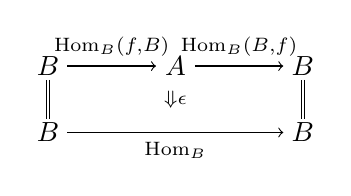
\begin{tikzpicture}[x=1em,y=1em]
  \node at (0,1.2)    {$B$};
  \node at (4.6,1.2)  {$A$};
  \node at (9.2,1.2)  {$B$};
  \node at (0,-1.2)   {$B$};
  \node at (9.2,-1.2) {$B$};
  \draw[->] (0.7,1.2)  -- node[above]{$\scriptstyle \mathrm{Hom}_{B}(f,B)$} (3.9,1.2);
  \draw[->] (5.3,1.2)  -- node[above]{$\scriptstyle \mathrm{Hom}_{B}(B,f)$} (8.5,1.2);
  \draw[->] (0.7,-1.2) -- node[below]{$\scriptstyle \mathrm{Hom}_{B}$} (8.5,-1.2);
  \draw[double] (0,0.7)   -- (0,-0.7);
  \draw[double] (9.2,0.7) -- (9.2,-0.7);
  \node at (4.6,0) {$\scriptstyle\Downarrow\epsilon$};
\end{tikzpicture}
\end{center}
它同时定义了 $B\xrightarrow{\mathrm{Hom}_{B}}B$ 穿过
$B\xrightarrow{\mathrm{Hom}_{B}(f,B)}A$ 的一个右扩张，以及
$B\xrightarrow{\mathrm{Hom}_{B}}B$ 穿过
$A\xrightarrow{\mathrm{Hom}_{B}(B,f)}B$ 的一个右提升。
\end{lemma}

\begin{proof}
二元胞腔 $\epsilon\colon \mathrm{Hom}_{B}(f,B)\divideontimes \mathrm{Hom}_{B}(B,f)\Rightarrow \mathrm{Hom}_{B}$（它也作为某种余单位出现在练习 8.4.v 中）在定理
8.4.4 与命题 8.2.4 的双射之下对应于一元单位胞腔 $\mathrm{Hom}_{f}$。
诸泛性质的验证留作\cref{ex:hom-cell-universal-properties}。
\end{proof}

\cref{lem:hom-binary-cell}的结果是一族更一般的例子之特例：

\begin{lemma}\label{lem:canonical-restriction-cells}
对任意模 $A\xrightarrow{E}B$ 与任意一对\trFunctor{} $g\colon C\to A$、
$f\colon D\to B$，诸典范\trCell
\begin{center}
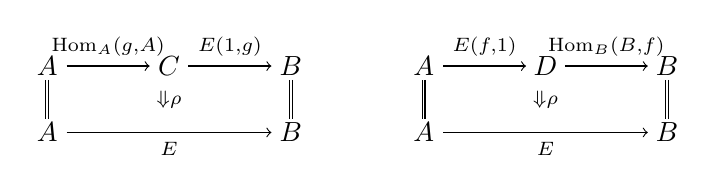
\begin{tikzpicture}[x=1em,y=1em]
  \begin{scope}
    \node at (0,1.2)   {$A$};
    \node at (4.4,1.2) {$C$};
    \node at (8.8,1.2) {$B$};
    \node at (0,-1.2)  {$A$};
    \node at (8.8,-1.2){$B$};
    \draw[->] (0.7,1.2)  -- node[above]{$\scriptstyle \mathrm{Hom}_{A}(g,A)$} (3.7,1.2);
    \draw[->] (5.1,1.2)  -- node[above]{$\scriptstyle E(1,g)$} (8.1,1.2);
    \draw[->] (0.7,-1.2) -- node[below]{$\scriptstyle E$} (8.1,-1.2);
    \draw[double] (0,0.7)   -- (0,-0.7);
    \draw[double] (8.8,0.7) -- (8.8,-0.7);
    \node at (4.4,0) {$\scriptstyle\Downarrow\rho$};
  \end{scope}
  \begin{scope}[shift={(13.6,0)}]
    \node at (0,1.2)   {$A$};
    \node at (4.4,1.2) {$D$};
    \node at (8.8,1.2) {$B$};
    \node at (0,-1.2)  {$A$};
    \node at (8.8,-1.2){$B$};
    \draw[->] (0.7,1.2)  -- node[above]{$\scriptstyle E(f,1)$} (3.7,1.2);
    \draw[->] (5.1,1.2)  -- node[above]{$\scriptstyle \mathrm{Hom}_{B}(B,f)$} (8.1,1.2);
    \draw[->] (0.7,-1.2) -- node[below]{$\scriptstyle E$} (8.1,-1.2);
    \draw[double] (0,0.7)   -- (0,-0.7);
    \draw[double] (8.8,0.7) -- (8.8,-0.7);
    \node at (4.4,0) {$\scriptstyle\Downarrow\rho$};
  \end{scope}
\end{tikzpicture}
\end{center}
展现 $E(1,g)$ 为 $E$ 穿过 $\mathrm{Hom}_{A}(g,A)$ 的右扩张，并展现 $E(f,1)$
为 $E$ 穿过 $\mathrm{Hom}_{B}(B,f)$ 的右提升。
\end{lemma}

\begin{proof}
所述的诸典范\trCell{}定义为：把定理 8.4.4 的双射作用于命题 8.2.1 的诸限制%
\trCell{}；也就是说，就上方左图所示的右扩张图表而言，这个\trCell{}作为如下
复合而得到
\begin{center}
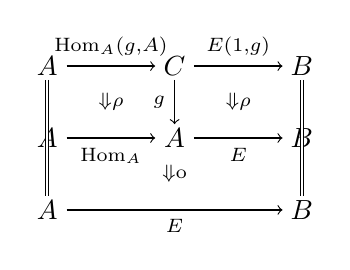
\begin{tikzpicture}[x=1em,y=1em]
  \node at (0,2.6)    {$A$};
  \node at (4.6,2.6)  {$C$};
  \node at (9.2,2.6)  {$B$};
  \node at (0,0)      {$A$};
  \node at (4.6,0)    {$A$};
  \node at (9.2,0)    {$B$};
  \node at (0,-2.6)   {$A$};
  \node at (9.2,-2.6) {$B$};
  \draw[->] (0.7,2.6)  -- node[above]{$\scriptstyle \mathrm{Hom}_{A}(g,A)$} (3.9,2.6);
  \draw[->] (5.3,2.6)  -- node[above]{$\scriptstyle E(1,g)$} (8.5,2.6);
  \draw[->] (0.7,0)    -- node[below]{$\scriptstyle \mathrm{Hom}_{A}$} (3.9,0);
  \draw[->] (5.3,0)    -- node[below]{$\scriptstyle E$} (8.5,0);
  \draw[->] (0.7,-2.6) -- node[below]{$\scriptstyle E$} (8.5,-2.6);
  \draw[double] (0,2.1)   -- (0,-2.1);
  \draw[double] (9.2,2.1) -- (9.2,-2.1);
  \draw[->] (4.6,2.1) -- node[left]{$\scriptstyle g$} (4.6,0.5);
  \node at (2.3,1.3)  {$\scriptstyle\Downarrow\rho$};
  \node at (6.9,1.3)  {$\scriptstyle\Downarrow\rho$};
  \node at (4.6,-1.3) {$\scriptstyle\Downarrow\mathrm{o}$};
\end{tikzpicture}
\end{center}
右扩张的泛性质由推论 8.4.6 提供。
\end{proof}

特别地：

\begin{corollary}\label{cor:module-self-extension}
任何模 $A\xrightarrow{E}B$ 都是它自身沿 $A\xrightarrow{\mathrm{Hom}_{A}}A$ 的
右扩张，同时也是它自身穿过 $B\xrightarrow{\mathrm{Hom}_{B}}B$ 的右提升。
\end{corollary}

诸右扩张与诸右提升分别可以理解为「在左侧与一支模作水平复合」和「在右侧与
一支模作水平复合」这两种运算的右伴随（见定理 12.3.6）。
由此引出下面这个「结合性」结果；我们就右扩张来陈述它，把右提升的对偶结果
留给读者。

\begin{proposition}\label{prop:right-extension-associativity}
设 $A\xrightarrow{K}B$、$B\xrightarrow{H}C$ 与 $A\xrightarrow{F}D$ 都是模，
使得复合 $K\otimes H$ 与右扩张 $B\xrightarrow{R_{K}F}D$ 存在。此时，
$R_{K}F$ 沿 $H$ 的右扩张存在，当且仅当 $F$ 沿 $K\otimes H$ 的右扩张存在；
而在二者存在时，$R_{H}(R_{K}F)\simeq_{C\times D}R_{K\otimes H}F$。
\end{proposition}

\begin{proof}
二元复合\trCell{} $\mu\colon K\divideontimes H\Rightarrow K\otimes H$ 的泛性质与右
扩张\trCell{} $\nu\colon K\divideontimes R_{K}F\Rightarrow F$ 一起，在涉及从 $C$ 到
$D$ 的模的任意相容序列 $R_{1}\divideontimes\cdots\divideontimes R_{n}$ 的诸\trCell{}之间
提供了如下双射（见记号 8.2.7）：
\begin{center}
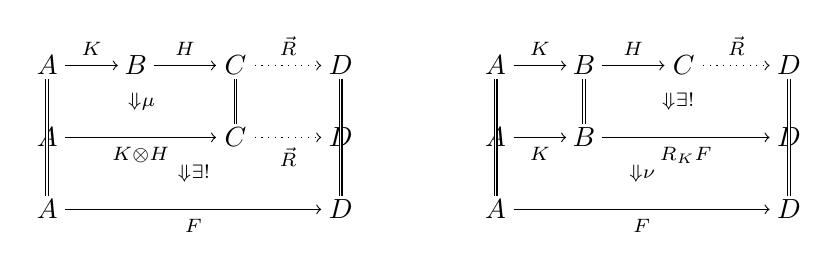
\begin{tikzpicture}[x=1em,y=1em]
  \begin{scope}
    \node at (0,2.6)    {$A$};
    \node at (3.2,2.6)  {$B$};
    \node at (6.8,2.6)  {$C$};
    \node at (10.6,2.6) {$D$};
    \draw[->] (0.65,2.6) -- node[above]{$\scriptstyle K$} (2.55,2.6);
    \draw[->] (3.85,2.6) -- node[above]{$\scriptstyle H$} (6.1,2.6);
    \draw[->,dotted] (7.5,2.6) -- node[above]{$\scriptstyle\vec{R}$} (9.9,2.6);
    \node at (0,0)    {$A$};
    \node at (6.8,0)  {$C$};
    \node at (10.6,0) {$D$};
    \draw[->] (0.65,0) -- node[below]{$\scriptstyle K\otimes H$} (6.1,0);
    \draw[->,dotted] (7.5,0) -- node[below]{$\scriptstyle\vec{R}$} (9.9,0);
    \node at (0,-2.6)   {$A$};
    \node at (10.6,-2.6){$D$};
    \draw[->] (0.65,-2.6) -- node[below]{$\scriptstyle F$} (9.9,-2.6);
    \draw[double] (0,2.1)    -- (0,-2.1);
    \draw[double] (10.6,2.1) -- (10.6,-2.1);
    \draw[double] (6.8,2.1)  -- (6.8,0.5);
    \node at (3.4,1.3)  {$\scriptstyle\Downarrow\mu$};
    \node at (5.3,-1.3) {$\scriptstyle\Downarrow\exists!$};
  \end{scope}
  \node at (13.4,0) {$\leftrightsquigarrow$};
  \begin{scope}[shift={(16.2,0)}]
    \node at (0,2.6)    {$A$};
    \node at (3.2,2.6)  {$B$};
    \node at (6.8,2.6)  {$C$};
    \node at (10.6,2.6) {$D$};
    \draw[->] (0.65,2.6) -- node[above]{$\scriptstyle K$} (2.55,2.6);
    \draw[->] (3.85,2.6) -- node[above]{$\scriptstyle H$} (6.1,2.6);
    \draw[->,dotted] (7.5,2.6) -- node[above]{$\scriptstyle\vec{R}$} (9.9,2.6);
    \node at (0,0)    {$A$};
    \node at (3.2,0)  {$B$};
    \node at (10.6,0) {$D$};
    \draw[->] (0.65,0) -- node[below]{$\scriptstyle K$} (2.55,0);
    \draw[->] (3.85,0) -- node[below]{$\scriptstyle R_{K}F$} (9.9,0);
    \node at (0,-2.6)   {$A$};
    \node at (10.6,-2.6){$D$};
    \draw[->] (0.65,-2.6) -- node[below]{$\scriptstyle F$} (9.9,-2.6);
    \draw[double] (0,2.1)    -- (0,-2.1);
    \draw[double] (10.6,2.1) -- (10.6,-2.1);
    \draw[double] (3.2,2.1)  -- (3.2,0.5);
    \node at (6.6,1.3)  {$\scriptstyle\Downarrow\exists!$};
    \node at (5.3,-1.3) {$\scriptstyle\Downarrow\nu$};
  \end{scope}
\end{tikzpicture}
\end{center}

在模的空序列的情形，这一双射在纤维化模映射 $K\otimes H\Rightarrow F$ 与纤维化
模映射 $H\Rightarrow R_{K}F$ 之间编码了一种伴随性。
若右扩张 $R_{K\otimes H}F$ 存在，我们就取它充当 $R$，并利用左下方的
二元\trCell{}去诱导右上方的二元\trCell{}；可以证明，这使得 $R_{K\otimes H}F$
表现为 $R_{K}F$ 沿 $H$ 的右扩张 $R_{H}(R_{K}F)$。
反之，若右扩张 $R_{H}(R_{K}F)$ 存在，我们就利用右上方的二元\trCell{}去诱导
左下方的二元\trCell{}；可以证明，这使得 $R_{H}(R_{K}F)$ 表现为 $F$ 沿
$K\otimes H$ 的右扩张 $R_{K\otimes H}F$。这种泛性质的转移是直截了当的，同样
由刚才展示的双射得出。

最后，若右扩张 $R_{H}(R_{K}F)$ 与 $R_{K\otimes H}F$ 分别已知存在，则上面的
论证结合右扩张的唯一性，便共同表明：作为从 $C$ 到 $D$ 的模，
$R_{K\otimes H}F\simeq R_{H}(R_{K}F)$（见\cref{ex:uniqueness-right-extensions}）。
\end{proof}

现在我们来说明\cref{def:right-extension-lifting-modules}如何经由定义 8.4.12
的共变嵌入与反变嵌入而与\cref{def:two-categorical-extension}相关联。

\begin{lemma}\label{lem:embedded-extension-lifting}
若
\begin{center}
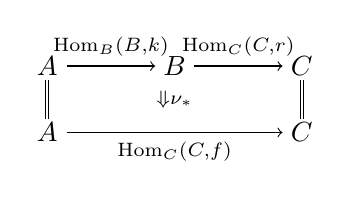
\begin{tikzpicture}[x=1em,y=1em]
  \node at (0,1.2)    {$A$};
  \node at (4.6,1.2)  {$B$};
  \node at (9.2,1.2)  {$C$};
  \node at (0,-1.2)   {$A$};
  \node at (9.2,-1.2) {$C$};
  \draw[->] (0.7,1.2)  -- node[above]{$\scriptstyle \mathrm{Hom}_{B}(B,k)$} (3.9,1.2);
  \draw[->] (5.3,1.2)  -- node[above]{$\scriptstyle \mathrm{Hom}_{C}(C,r)$} (8.5,1.2);
  \draw[->] (0.7,-1.2) -- node[below]{$\scriptstyle \mathrm{Hom}_{C}(C,f)$} (8.5,-1.2);
  \draw[double] (0,0.7)   -- (0,-0.7);
  \draw[double] (9.2,0.7) -- (9.2,-0.7);
  \node at (4.6,0) {$\scriptstyle\Downarrow\nu_{*}$};
\end{tikzpicture}
\end{center}
在模的\trVirtualEquipment{}中定义一个右扩张，则 $\nu\colon rk\Rightarrow f$ 在%
\trHomotopyTwoCategory{}中定义一个右扩张。对偶地，若
\begin{center}
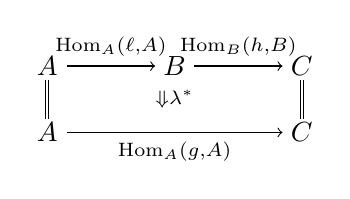
\begin{tikzpicture}[x=1em,y=1em]
  \node at (0,1.2)    {$A$};
  \node at (4.6,1.2)  {$B$};
  \node at (9.2,1.2)  {$C$};
  \node at (0,-1.2)   {$A$};
  \node at (9.2,-1.2) {$C$};
  \draw[->] (0.7,1.2)  -- node[above]{$\scriptstyle \mathrm{Hom}_{A}(\ell,A)$} (3.9,1.2);
  \draw[->] (5.3,1.2)  -- node[above]{$\scriptstyle \mathrm{Hom}_{B}(h,B)$} (8.5,1.2);
  \draw[->] (0.7,-1.2) -- node[below]{$\scriptstyle \mathrm{Hom}_{A}(g,A)$} (8.5,-1.2);
  \draw[double] (0,0.7)   -- (0,-0.7);
  \draw[double] (9.2,0.7) -- (9.2,-0.7);
  \node at (4.6,0) {$\scriptstyle\Downarrow\lambda^{*}$};
\end{tikzpicture}
\end{center}
在模的\trVirtualEquipment{}中定义一个右提升，则 $\lambda\colon g\Rightarrow \ell h$
是\trHomotopyTwoCategory{}中的一个左扩张。
\end{lemma}

\begin{proof}
由推论 8.4.9，二元\trCell{} $\nu_{*}\colon \mathrm{Hom}_{B}(B,k)\divideontimes\mathrm{Hom}_{C}(C,r)\Rightarrow \mathrm{Hom}_{C}(C,f)$ 对应于一元\trCell{}
$\nu_{*}\colon \mathrm{Hom}_{C}(C,rk)\Rightarrow \mathrm{Hom}_{C}(C,f)$；再由
命题 8.4.11，后者对应于\trHomotopyTwoCategory{}中的\trNaturalTransformation{}
$\nu\colon rk\Rightarrow f$。
在这一对应之下，限制到右可表示模时，\cref{def:right-extension-lifting-modules}
的泛性质显然涵盖了\cref{def:two-categorical-extension}的泛性质。
左扩张情形类似，经由定义 8.4.12 的反变嵌入。
\end{proof}

对于共变嵌入之像中的模右扩张图表，一个更精细的刻画出现在定理 9.3.3 中；但共变
嵌入之像中的模右提升图表，我们现在就能刻画。
请回忆定义 2.3.5 中引入的绝对右提升图表概念。

\begin{proposition}\label{prop:absolute-vs-module-lifting}
\trInfinityCosmos{}的\trHomotopyTwoCategory{}中如下左图所示的一个%
\trNaturalTransformation{}定义一个绝对右提升图表，当且仅当如下右图所示的那个
对应的二元\trCell{}在模的\trVirtualEquipment{}中定义一个右提升：
\begin{center}
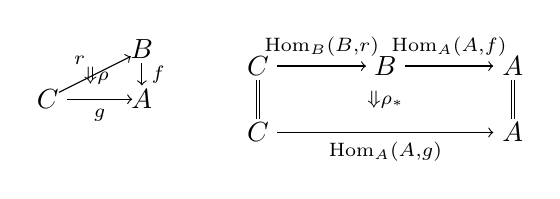
\begin{tikzpicture}[x=1em,y=1em]
  \node at (0,0)     {$C$};
  \node at (3.4,1.8) {$B$};
  \node at (3.4,0)   {$A$};
  \draw[->] (0.4,0.25) -- node[above left,pos=0.5]{$\scriptstyle r$} (3.0,1.55);
  \draw[->] (3.4,1.3)  -- node[right]{$\scriptstyle f$} (3.4,0.5);
  \draw[->] (0.7,0)    -- node[below]{$\scriptstyle g$} (3.05,0);
  \node at (1.75,0.85) {$\scriptstyle\Downarrow\rho$};
  \node at (5.9,0.85)  {$\leftrightsquigarrow$};
  \begin{scope}[shift={(7.6,0)}]
    \node at (0,1.2)    {$C$};
    \node at (4.6,1.2)  {$B$};
    \node at (9.2,1.2)  {$A$};
    \node at (0,-1.2)   {$C$};
    \node at (9.2,-1.2) {$A$};
    \draw[->] (0.7,1.2)  -- node[above]{$\scriptstyle \mathrm{Hom}_{B}(B,r)$} (3.9,1.2);
    \draw[->] (5.3,1.2)  -- node[above]{$\scriptstyle \mathrm{Hom}_{A}(A,f)$} (8.5,1.2);
    \draw[->] (0.7,-1.2) -- node[below]{$\scriptstyle \mathrm{Hom}_{A}(A,g)$} (8.5,-1.2);
    \draw[double] (0,0.7)   -- (0,-0.7);
    \draw[double] (9.2,0.7) -- (9.2,-0.7);
    \node at (4.6,0) {$\scriptstyle\Downarrow\rho_{*}$};
  \end{scope}
\end{tikzpicture}
\end{center}
对偶地，\trInfinityCosmos{}的\trHomotopyTwoCategory{}中如下左图所示的一个
2-\trCell{}定义一个绝对左提升图表，当且仅当如下右图所示的那个对应的二元%
\trCell{}在模的\trVirtualEquipment{}中定义一个右扩张：\footnote{原书印作
「$A$」，按模方向的型算应为 $C$，此处径改。——译者注}
\begin{center}
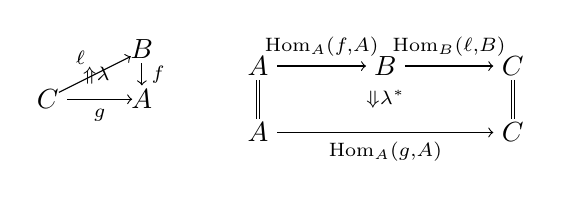
\begin{tikzpicture}[x=1em,y=1em]
  \node at (0,0)     {$C$};
  \node at (3.4,1.8) {$B$};
  \node at (3.4,0)   {$A$};
  \draw[->] (0.4,0.25) -- node[above left,pos=0.5]{$\scriptstyle\ell$} (3.0,1.55);
  \draw[->] (3.4,1.3)  -- node[right]{$\scriptstyle f$} (3.4,0.5);
  \draw[->] (0.7,0)    -- node[below]{$\scriptstyle g$} (3.05,0);
  \node at (1.75,0.85) {$\scriptstyle\Uparrow\lambda$};
  \node at (5.9,0.85)  {$\leftrightsquigarrow$};
  \begin{scope}[shift={(7.6,0)}]
    \node at (0,1.2)    {$A$};
    \node at (4.6,1.2)  {$B$};
    \node at (9.2,1.2)  {$C$};
    \node at (0,-1.2)   {$A$};
    \node at (9.2,-1.2) {$C$};
    \draw[->] (0.7,1.2)  -- node[above]{$\scriptstyle \mathrm{Hom}_{A}(f,A)$} (3.9,1.2);
    \draw[->] (5.3,1.2)  -- node[above]{$\scriptstyle \mathrm{Hom}_{B}(\ell,B)$} (8.5,1.2);
    \draw[->] (0.7,-1.2) -- node[below]{$\scriptstyle \mathrm{Hom}_{A}(g,A)$} (8.5,-1.2);
    \draw[double] (0,0.7)   -- (0,-0.7);
    \draw[double] (9.2,0.7) -- (9.2,-0.7);
    \node at (4.6,0) {$\scriptstyle\Downarrow\lambda^{*}$};
  \end{scope}
\end{tikzpicture}
\end{center}
\end{proposition}

\begin{proof}
由命题 8.4.11，\trInfinityCosmos{}的\trHomotopyTwoCategory{}中的诸%
\trNaturalTransformation{}与模的\trVirtualEquipment{}中各种形状的一元方块
一一对应。
由这一结果以及推论 8.4.6 与推论 8.4.9，存在诸典范双射：
\begin{rveq}\label{eq:canonical-bijections}
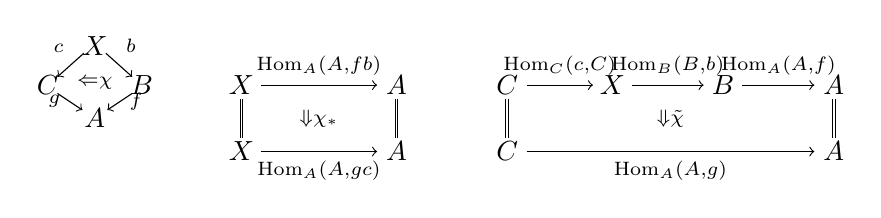
\begin{tikzpicture}[x=1em,y=1em]
  \node at (1.7,2.6) {$X$};
  \node at (0,1.2)   {$C$};
  \node at (3.4,1.2) {$B$};
  \node at (1.7,0)   {$A$};
  \draw[->] (2.1,2.35) -- node[above right,pos=0.4]{$\scriptstyle b$} (3.05,1.5);
  \draw[->] (1.3,2.35) -- node[above left,pos=0.4]{$\scriptstyle c$} (0.35,1.5);
  \draw[->] (3.05,0.9) -- node[right,pos=0.5]{$\scriptstyle f$} (2.15,0.3);
  \draw[->] (0.35,0.9) -- node[left,pos=0.5]{$\scriptstyle g$} (1.25,0.3);
  \node at (1.7,1.25) {$\scriptstyle\Leftarrow\chi$};
  \node at (5.3,1.2)  {$\leftrightsquigarrow$};
  \begin{scope}[shift={(7.0,0)}]
    \node at (0,1.2)    {$X$};
    \node at (5.6,1.2)  {$A$};
    \node at (0,-1.2)   {$X$};
    \node at (5.6,-1.2) {$A$};
    \draw[->] (0.7,1.2)  -- node[above]{$\scriptstyle \mathrm{Hom}_{A}(A,fb)$} (4.9,1.2);
    \draw[->] (0.7,-1.2) -- node[below]{$\scriptstyle \mathrm{Hom}_{A}(A,gc)$} (4.9,-1.2);
    \draw[double] (0,0.7)   -- (0,-0.7);
    \draw[double] (5.6,0.7) -- (5.6,-0.7);
    \node at (2.8,0) {$\scriptstyle\Downarrow\chi_{*}$};
  \end{scope}
  \node at (14.6,1.2) {$\leftrightsquigarrow$};
  \begin{scope}[shift={(16.6,0)}]
    \node at (0,1.2)    {$C$};
    \node at (3.8,1.2)  {$X$};
    \node at (7.8,1.2)  {$B$};
    \node at (11.8,1.2) {$A$};
    \node at (0,-1.2)   {$C$};
    \node at (11.8,-1.2){$A$};
    \draw[->] (0.7,1.2)  -- node[above]{$\scriptstyle \mathrm{Hom}_{C}(c,C)$} (3.1,1.2);
    \draw[->] (4.5,1.2)  -- node[above]{$\scriptstyle \mathrm{Hom}_{B}(B,b)$} (7.1,1.2);
    \draw[->] (8.5,1.2)  -- node[above]{$\scriptstyle \mathrm{Hom}_{A}(A,f)$} (11.1,1.2);
    \draw[->] (0.7,-1.2) -- node[below]{$\scriptstyle \mathrm{Hom}_{A}(A,g)$} (11.1,-1.2);
    \draw[double] (0,0.7)    -- (0,-0.7);
    \draw[double] (11.8,0.7) -- (11.8,-0.7);
    \node at (5.9,0) {$\scriptstyle\Downarrow\tilde{\chi}$};
  \end{scope}
\end{tikzpicture}
\end{rveq}

若二元\trCell{} $\rho_{*}\colon \mathrm{Hom}_{B}(B,r)\divideontimes\mathrm{Hom}_{A}(A,f)\Rightarrow \mathrm{Hom}_{A}(A,g)$ 在模的%
\trVirtualEquipment{}中定义一个右提升图表，则存在唯一的分解
\begin{center}
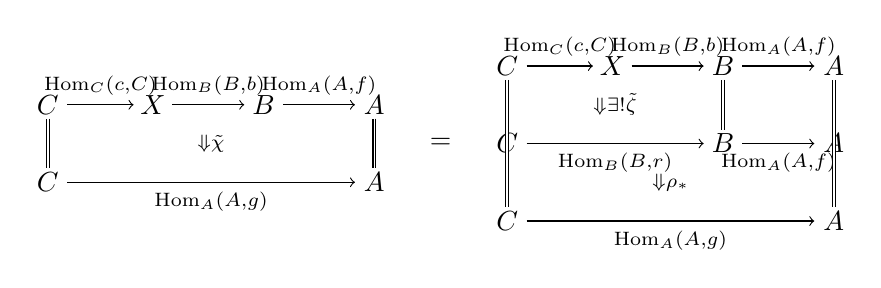
\begin{tikzpicture}[x=1em,y=1em]
  \begin{scope}
    \node at (0,1.4)    {$C$};
    \node at (3.8,1.4)  {$X$};
    \node at (7.8,1.4)  {$B$};
    \node at (11.8,1.4) {$A$};
    \node at (0,-1.4)   {$C$};
    \node at (11.8,-1.4){$A$};
    \draw[->] (0.7,1.4)  -- node[above]{$\scriptstyle \mathrm{Hom}_{C}(c,C)$} (3.1,1.4);
    \draw[->] (4.5,1.4)  -- node[above]{$\scriptstyle \mathrm{Hom}_{B}(B,b)$} (7.1,1.4);
    \draw[->] (8.5,1.4)  -- node[above]{$\scriptstyle \mathrm{Hom}_{A}(A,f)$} (11.1,1.4);
    \draw[->] (0.7,-1.4) -- node[below]{$\scriptstyle \mathrm{Hom}_{A}(A,g)$} (11.1,-1.4);
    \draw[double] (0,0.9)    -- (0,-0.9);
    \draw[double] (11.8,0.9) -- (11.8,-0.9);
    \node at (5.9,0) {$\scriptstyle\Downarrow\tilde{\chi}$};
  \end{scope}
  \node at (14.2,0) {$=$};
  \begin{scope}[shift={(16.6,0)}]
    \node at (0,2.8)    {$C$};
    \node at (3.8,2.8)  {$X$};
    \node at (7.8,2.8)  {$B$};
    \node at (11.8,2.8) {$A$};
    \draw[->] (0.7,2.8)  -- node[above]{$\scriptstyle \mathrm{Hom}_{C}(c,C)$} (3.1,2.8);
    \draw[->] (4.5,2.8)  -- node[above]{$\scriptstyle \mathrm{Hom}_{B}(B,b)$} (7.1,2.8);
    \draw[->] (8.5,2.8)  -- node[above]{$\scriptstyle \mathrm{Hom}_{A}(A,f)$} (11.1,2.8);
    \node at (0,0)    {$C$};
    \node at (7.8,0)  {$B$};
    \node at (11.8,0) {$A$};
    \draw[->] (0.7,0) -- node[below]{$\scriptstyle \mathrm{Hom}_{B}(B,r)$} (7.1,0);
    \draw[->] (8.5,0) -- node[below]{$\scriptstyle \mathrm{Hom}_{A}(A,f)$} (11.1,0);
    \node at (0,-2.8)   {$C$};
    \node at (11.8,-2.8){$A$};
    \draw[->] (0.7,-2.8) -- node[below]{$\scriptstyle \mathrm{Hom}_{A}(A,g)$} (11.1,-2.8);
    \draw[double] (0,2.3)    -- (0,-2.3);
    \draw[double] (11.8,2.3) -- (11.8,-2.3);
    \draw[double] (7.8,2.3)  -- (7.8,0.5);
    \node at (3.9,1.4)  {$\scriptstyle\Downarrow\exists!\tilde{\zeta}$};
    \node at (5.9,-1.4) {$\scriptstyle\Downarrow\rho_{*}$};
  \end{scope}
\end{tikzpicture}
\end{center}
反转 \eqref{eq:canonical-bijections} 的典范双射，这就定义了%
\trHomotopyTwoCategory{}中所要的那个唯一分解：
\begin{center}
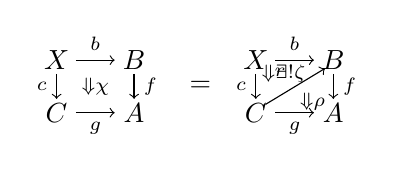
\begin{tikzpicture}[x=1em,y=1em]
  \node at (0,1.9)   {$X$};
  \node at (2.8,1.9) {$B$};
  \node at (0,0)     {$C$};
  \node at (2.8,0)   {$A$};
  \draw[->] (0.7,1.9) -- node[above]{$\scriptstyle b$} (2.1,1.9);
  \draw[->] (0,1.4)   -- node[left]{$\scriptstyle c$} (0,0.5);
  \draw[->] (2.8,1.4) -- node[right]{$\scriptstyle f$} (2.8,0.5);
  \draw[->] (0.7,0)   -- node[below]{$\scriptstyle g$} (2.1,0);
  \node at (1.4,0.95) {$\scriptstyle\Downarrow\chi$};
  \node at (5.2,0.95) {$=$};
  \begin{scope}[shift={(7.2,0)}]
    \node at (0,1.9)   {$X$};
    \node at (2.8,1.9) {$B$};
    \node at (0,0)     {$C$};
    \node at (2.8,0)   {$A$};
    \draw[->] (0.7,1.9) -- node[above]{$\scriptstyle b$} (2.1,1.9);
    \draw[->] (0,1.4)   -- node[left]{$\scriptstyle c$} (0,0.5);
    \draw[->] (2.8,1.4) -- node[right]{$\scriptstyle f$} (2.8,0.5);
    \draw[->] (0.7,0)   -- node[below]{$\scriptstyle g$} (2.1,0);
    \draw[->] (0.35,0.3) -- node[above left,pos=0.5]{$\scriptstyle r$} (2.5,1.6);
    \node at (1.0,1.4)  {$\scriptstyle\Downarrow\exists!\zeta$};
    \node at (2.05,0.4) {$\scriptstyle\Downarrow\rho$};
  \end{scope}
\end{tikzpicture}
\end{center}
于是，若 $\rho_{*}\colon \mathrm{Hom}_{B}(B,r)\divideontimes \mathrm{Hom}_{A}(A,f)\Rightarrow \mathrm{Hom}_{A}(A,g)$ 是一个右提升，则 $\rho\colon fr\Rightarrow g$
是一个绝对右提升。

反之，设 $\rho\colon fr\Rightarrow g$ 是一个绝对右提升，并考虑模的%
\trVirtualEquipment{}中如下形状的一个\trCell{}：
\begin{center}
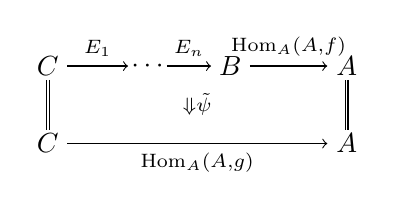
\begin{tikzpicture}[x=1em,y=1em]
  \node at (0,1.4)    {$C$};
  \node at (3.6,1.4)  {$\cdots$};
  \node at (6.6,1.4)  {$B$};
  \node at (10.8,1.4) {$A$};
  \node at (0,-1.4)   {$C$};
  \node at (10.8,-1.4){$A$};
  \draw[->] (0.7,1.4)  -- node[above]{$\scriptstyle E_{1}$} (2.9,1.4);
  \draw[->] (4.3,1.4)  -- node[above]{$\scriptstyle E_{n}$} (5.9,1.4);
  \draw[->] (7.3,1.4)  -- node[above]{$\scriptstyle \mathrm{Hom}_{A}(A,f)$} (10.1,1.4);
  \draw[->] (0.7,-1.4) -- node[below]{$\scriptstyle \mathrm{Hom}_{A}(A,g)$} (10.1,-1.4);
  \draw[double] (0,0.9)    -- (0,-0.9);
  \draw[double] (10.8,0.9) -- (10.8,-0.9);
  \node at (5.4,0) {$\scriptstyle\Downarrow\tilde{\psi}$};
\end{tikzpicture}
\end{center}
令 $C\overset{q}{\twoheadleftarrow}\vec{E}\overset{p}{\twoheadrightarrow}B$ 表示
复合双侧纤维化 $E_{1}\divideontimes\cdots\divideontimes E_{n}$。
由注 8.3.12，模映射 $\tilde{\psi}\colon E_{1}\divideontimes\cdots\divideontimes E_{n}\divideontimes\mathrm{Hom}_{A}(A,f)\Rightarrow \mathrm{Hom}_{A}(A,g)$ 对应于模映射
$\hat{\psi}\colon \mathrm{Hom}_{C}(q,C)\divideontimes \mathrm{Hom}_{B}(B,p)\divideontimes\mathrm{Hom}_{A}(A,f)\Rightarrow \mathrm{Hom}_{A}(A,g)$，如下左图所示。

如 \eqref{eq:canonical-bijections} 中所论，这些模映射与如下中图所示的诸%
\trNaturalTransformation{}处于一个典范双射之中：
\begin{center}
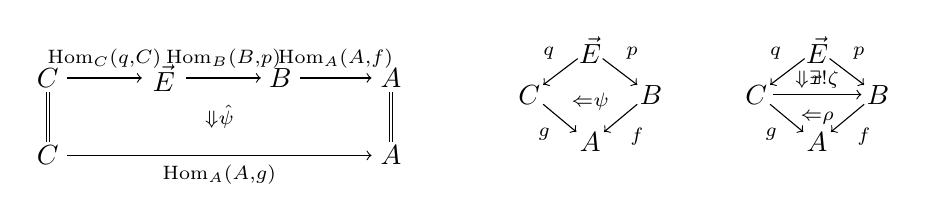
\begin{tikzpicture}[x=1em,y=1em]
  \begin{scope}
    \node at (0,1.4)    {$C$};
    \node at (4.2,1.4)  {$\vec{E}$};
    \node at (8.4,1.4)  {$B$};
    \node at (12.4,1.4) {$A$};
    \node at (0,-1.4)   {$C$};
    \node at (12.4,-1.4){$A$};
    \draw[->] (0.7,1.4)  -- node[above]{$\scriptstyle \mathrm{Hom}_{C}(q,C)$} (3.4,1.4);
    \draw[->] (5.0,1.4)  -- node[above]{$\scriptstyle \mathrm{Hom}_{B}(B,p)$} (7.7,1.4);
    \draw[->] (9.1,1.4)  -- node[above]{$\scriptstyle \mathrm{Hom}_{A}(A,f)$} (11.7,1.4);
    \draw[->] (0.7,-1.4) -- node[below]{$\scriptstyle \mathrm{Hom}_{A}(A,g)$} (11.7,-1.4);
    \draw[double] (0,0.9)    -- (0,-0.9);
    \draw[double] (12.4,0.9) -- (12.4,-0.9);
    \node at (6.2,0) {$\scriptstyle\Downarrow\hat{\psi}$};
  \end{scope}
  \node at (15.0,0) {$\leftrightsquigarrow$};
  \begin{scope}[shift={(17.4,0)}]
    \node at (2.2,2.4)  {$\vec{E}$};
    \node at (0,0.8)    {$C$};
    \node at (4.4,0.8)  {$B$};
    \node at (2.2,-0.9) {$A$};
    \draw[->] (1.75,2.1) -- node[above left,pos=0.4]{$\scriptstyle q$} (0.5,1.15);
    \draw[->] (2.65,2.1) -- node[above right,pos=0.4]{$\scriptstyle p$} (3.9,1.15);
    \draw[->] (0.5,0.45) -- node[below left,pos=0.5]{$\scriptstyle g$} (1.7,-0.55);
    \draw[->] (3.9,0.45) -- node[below right,pos=0.5]{$\scriptstyle f$} (2.7,-0.55);
    \node at (2.2,0.55) {$\scriptstyle\Leftarrow\psi$};
  \end{scope}
  \node at (23.2,0) {$\leftrightsquigarrow$};
  \begin{scope}[shift={(25.6,0)}]
    \node at (2.2,2.4)  {$\vec{E}$};
    \node at (0,0.8)    {$C$};
    \node at (4.4,0.8)  {$B$};
    \node at (2.2,-0.9) {$A$};
    \draw[->] (1.75,2.1) -- node[above left,pos=0.4]{$\scriptstyle q$} (0.5,1.15);
    \draw[->] (2.65,2.1) -- node[above right,pos=0.4]{$\scriptstyle p$} (3.9,1.15);
    \draw[->] (0.6,0.8)  -- node[above]{$\scriptstyle r$} (3.8,0.8);
    \draw[->] (0.5,0.45) -- node[below left,pos=0.5]{$\scriptstyle g$} (1.7,-0.55);
    \draw[->] (3.9,0.45) -- node[below right,pos=0.5]{$\scriptstyle f$} (2.7,-0.55);
    \node at (2.2,1.35)  {$\scriptstyle\Downarrow\exists!\zeta$};
    \node at (2.2,-0.05) {$\scriptstyle\Leftarrow\rho$};
  \end{scope}
\end{tikzpicture}
\end{center}
由于 $\rho\colon fr\Rightarrow g$ 被假定为绝对右提升，$\psi$ 经由 $\rho$ 唯一地
分解，从而如上右图那样定义了一个对应的 2-\trCell{} $\zeta\colon p\Rightarrow rq$。
再度应用 \eqref{eq:canonical-bijections}，这就构造出模的
\trVirtualEquipment{}中的一个唯一分解
\begin{center}
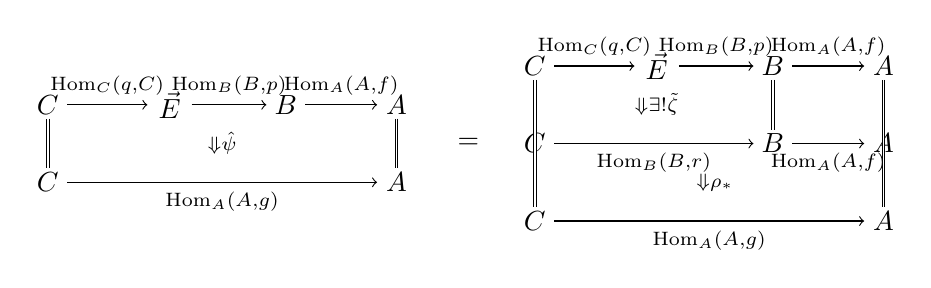
\begin{tikzpicture}[x=1em,y=1em]
  \begin{scope}
    \node at (0,1.4)    {$C$};
    \node at (4.4,1.4)  {$\vec{E}$};
    \node at (8.6,1.4)  {$B$};
    \node at (12.6,1.4) {$A$};
    \node at (0,-1.4)   {$C$};
    \node at (12.6,-1.4){$A$};
    \draw[->] (0.7,1.4)  -- node[above]{$\scriptstyle \mathrm{Hom}_{C}(q,C)$} (3.6,1.4);
    \draw[->] (5.2,1.4)  -- node[above]{$\scriptstyle \mathrm{Hom}_{B}(B,p)$} (7.9,1.4);
    \draw[->] (9.3,1.4)  -- node[above]{$\scriptstyle \mathrm{Hom}_{A}(A,f)$} (11.9,1.4);
    \draw[->] (0.7,-1.4) -- node[below]{$\scriptstyle \mathrm{Hom}_{A}(A,g)$} (11.9,-1.4);
    \draw[double] (0,0.9)    -- (0,-0.9);
    \draw[double] (12.6,0.9) -- (12.6,-0.9);
    \node at (6.3,0) {$\scriptstyle\Downarrow\hat{\psi}$};
  \end{scope}
  \node at (15.2,0) {$=$};
  \begin{scope}[shift={(17.6,0)}]
    \node at (0,2.8)    {$C$};
    \node at (4.4,2.8)  {$\vec{E}$};
    \node at (8.6,2.8)  {$B$};
    \node at (12.6,2.8) {$A$};
    \draw[->] (0.7,2.8)  -- node[above]{$\scriptstyle \mathrm{Hom}_{C}(q,C)$} (3.6,2.8);
    \draw[->] (5.2,2.8)  -- node[above]{$\scriptstyle \mathrm{Hom}_{B}(B,p)$} (7.9,2.8);
    \draw[->] (9.3,2.8)  -- node[above]{$\scriptstyle \mathrm{Hom}_{A}(A,f)$} (11.9,2.8);
    \node at (0,0)    {$C$};
    \node at (8.6,0)  {$B$};
    \node at (12.6,0) {$A$};
    \draw[->] (0.7,0) -- node[below]{$\scriptstyle \mathrm{Hom}_{B}(B,r)$} (7.9,0);
    \draw[->] (9.3,0) -- node[below]{$\scriptstyle \mathrm{Hom}_{A}(A,f)$} (11.9,0);
    \node at (0,-2.8)   {$C$};
    \node at (12.6,-2.8){$A$};
    \draw[->] (0.7,-2.8) -- node[below]{$\scriptstyle \mathrm{Hom}_{A}(A,g)$} (11.9,-2.8);
    \draw[double] (0,2.3)    -- (0,-2.3);
    \draw[double] (12.6,2.3) -- (12.6,-2.3);
    \draw[double] (8.6,2.3)  -- (8.6,0.5);
    \node at (4.4,1.4)  {$\scriptstyle\Downarrow\exists!\tilde{\zeta}$};
    \node at (6.5,-1.4) {$\scriptstyle\Downarrow\rho_{*}$};
  \end{scope}
\end{tikzpicture}
\end{center}
由注 8.3.12，这就定义了一个双射
\begin{center}
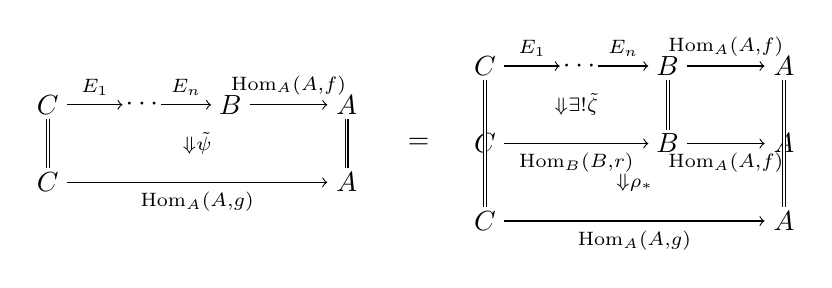
\begin{tikzpicture}[x=1em,y=1em]
  \begin{scope}
    \node at (0,1.4)    {$C$};
    \node at (3.4,1.4)  {$\cdots$};
    \node at (6.6,1.4)  {$B$};
    \node at (10.8,1.4) {$A$};
    \node at (0,-1.4)   {$C$};
    \node at (10.8,-1.4){$A$};
    \draw[->] (0.7,1.4)  -- node[above]{$\scriptstyle E_{1}$} (2.7,1.4);
    \draw[->] (4.1,1.4)  -- node[above]{$\scriptstyle E_{n}$} (5.9,1.4);
    \draw[->] (7.3,1.4)  -- node[above]{$\scriptstyle \mathrm{Hom}_{A}(A,f)$} (10.1,1.4);
    \draw[->] (0.7,-1.4) -- node[below]{$\scriptstyle \mathrm{Hom}_{A}(A,g)$} (10.1,-1.4);
    \draw[double] (0,0.9)    -- (0,-0.9);
    \draw[double] (10.8,0.9) -- (10.8,-0.9);
    \node at (5.4,0) {$\scriptstyle\Downarrow\tilde{\psi}$};
  \end{scope}
  \node at (13.4,0) {$=$};
  \begin{scope}[shift={(15.8,0)}]
    \node at (0,2.8)    {$C$};
    \node at (3.4,2.8)  {$\cdots$};
    \node at (6.6,2.8)  {$B$};
    \node at (10.8,2.8) {$A$};
    \draw[->] (0.7,2.8)  -- node[above]{$\scriptstyle E_{1}$} (2.7,2.8);
    \draw[->] (4.1,2.8)  -- node[above]{$\scriptstyle E_{n}$} (5.9,2.8);
    \draw[->] (7.3,2.8)  -- node[above]{$\scriptstyle \mathrm{Hom}_{A}(A,f)$} (10.1,2.8);
    \node at (0,0)    {$C$};
    \node at (6.6,0)  {$B$};
    \node at (10.8,0) {$A$};
    \draw[->] (0.7,0) -- node[below]{$\scriptstyle \mathrm{Hom}_{B}(B,r)$} (5.9,0);
    \draw[->] (7.3,0) -- node[below]{$\scriptstyle \mathrm{Hom}_{A}(A,f)$} (10.1,0);
    \node at (0,-2.8)   {$C$};
    \node at (10.8,-2.8){$A$};
    \draw[->] (0.7,-2.8) -- node[below]{$\scriptstyle \mathrm{Hom}_{A}(A,g)$} (10.1,-2.8);
    \draw[double] (0,2.3)    -- (0,-2.3);
    \draw[double] (10.8,2.3) -- (10.8,-2.3);
    \draw[double] (6.6,2.3)  -- (6.6,0.5);
    \node at (3.3,1.4)  {$\scriptstyle\Downarrow\exists!\tilde{\zeta}$};
    \node at (5.4,-1.4) {$\scriptstyle\Downarrow\rho_{*}$};
  \end{scope}
\end{tikzpicture}
\end{center}
于是，若 $\rho\colon fr\Rightarrow g$ 定义一个绝对右提升，则
$\rho_{*}\colon\mathrm{Hom}_{B}(B,r)\divideontimes \mathrm{Hom}_{A}(A,f)\Rightarrow\mathrm{Hom}_{A}(A,g)$
定义一个右提升。
\end{proof}

在定理 9.3.3 中我们将发现：共变嵌入之像中的那些模的右扩张，恰由%
\trHomotopyTwoCategory{}中所寻求的\emph{逐点}右扩张来刻画；对偶地，逐点左
扩张对应于反变嵌入之像中的那些模的右提升。在下一节中，我们将为这一概念的
2-范畴式定义逐步搭建基础。

\subsection*{练习}

\begin{exercise}\label{ex:uniqueness-right-extensions}
设 $B\xrightarrow{R}C$ 与 $B\xrightarrow{S}C$ 在\cref{def:right-extension-lifting-modules}
的意义下都定义了模 $A\xrightarrow{F}C$ 沿模 $A\xrightarrow{K}B$ 的一个右扩张。
请证明 $R\simeq_{B\times C}S$。
\end{exercise}

\begin{exercise}\label{ex:hom-cell-universal-properties}
不借助\cref{lem:canonical-restriction-cells}而完成\cref{lem:hom-binary-cell}
的证明。
\end{exercise}

\begin{exercise}\label{ex:closed-virtual-equipment}
一个\trVirtualEquipment{}是\textbf{封闭的}（closed），若\cref{def:right-extension-lifting-modules}
的右扩张与右提升总是存在。
在一个封闭\trVirtualEquipment{}中，请证明：一个\trCell{}
$\mu\colon E_{1}\divideontimes\cdots\divideontimes E_{n}\Rightarrow E$ 是一个复合，当且仅当沿 $\mu$ 的
限制对所有与 $E$ 平行的模 $F$ 都在纤维化一元\trCell{} $E\Rightarrow F$ 与
纤维化\trCell{} $E_{1}\divideontimes\cdots\divideontimes E_{n}\Rightarrow F$ 之间定义一个
双射。
\end{exercise}

\begin{exercise}\label{ex:right-liftings-through-composite}
将\cref{prop:right-extension-associativity}对偶化，以刻画穿过两支模之复合的
右提升。
\end{exercise}

\begin{exercise}\label{ex:dual-absolute-left-lifting}
建立\cref{prop:absolute-vs-module-lifting}的对偶：验证绝对左提升图表
$\lambda\colon g\Rightarrow f\ell$ 对应于右扩张图表
$\lambda^{*}\colon\mathrm{Hom}_{A}(f,A)\divideontimes \mathrm{Hom}_{B}(\ell,B)\Rightarrow\mathrm{Hom}_{A}(g,A)$。
\end{exercise}

